\begin{frame}\begin{center}
		\LARGE\textbf{Testing}
\end{center}\end{frame}
%-------------------------------------------------------------------------------
%-------------------------------------------------------------------------------
\begin{frame}
An important statistic for GMM is the test of overidentifying restrictions that is given by

\begin{align*}
T = n\,\hat{g}(\hat{\beta})^\prime \,\hat{\Sigma}^{-1}\,\hat{g}(\hat{\beta})
\end{align*}

which converges in distribution to

\begin{align*}
T \xrightarrow{d} \chi^2(m - p)
\end{align*}

under $H_0$ that the model is correctly specified.

\end{frame}
%-------------------------------------------------------------------------------
%-------------------------------------------------------------------------------
\begin{frame}
\begin{figure}[htp]\centering
\caption{Density of $\chi^2(2)$}
\scalebox{0.75}{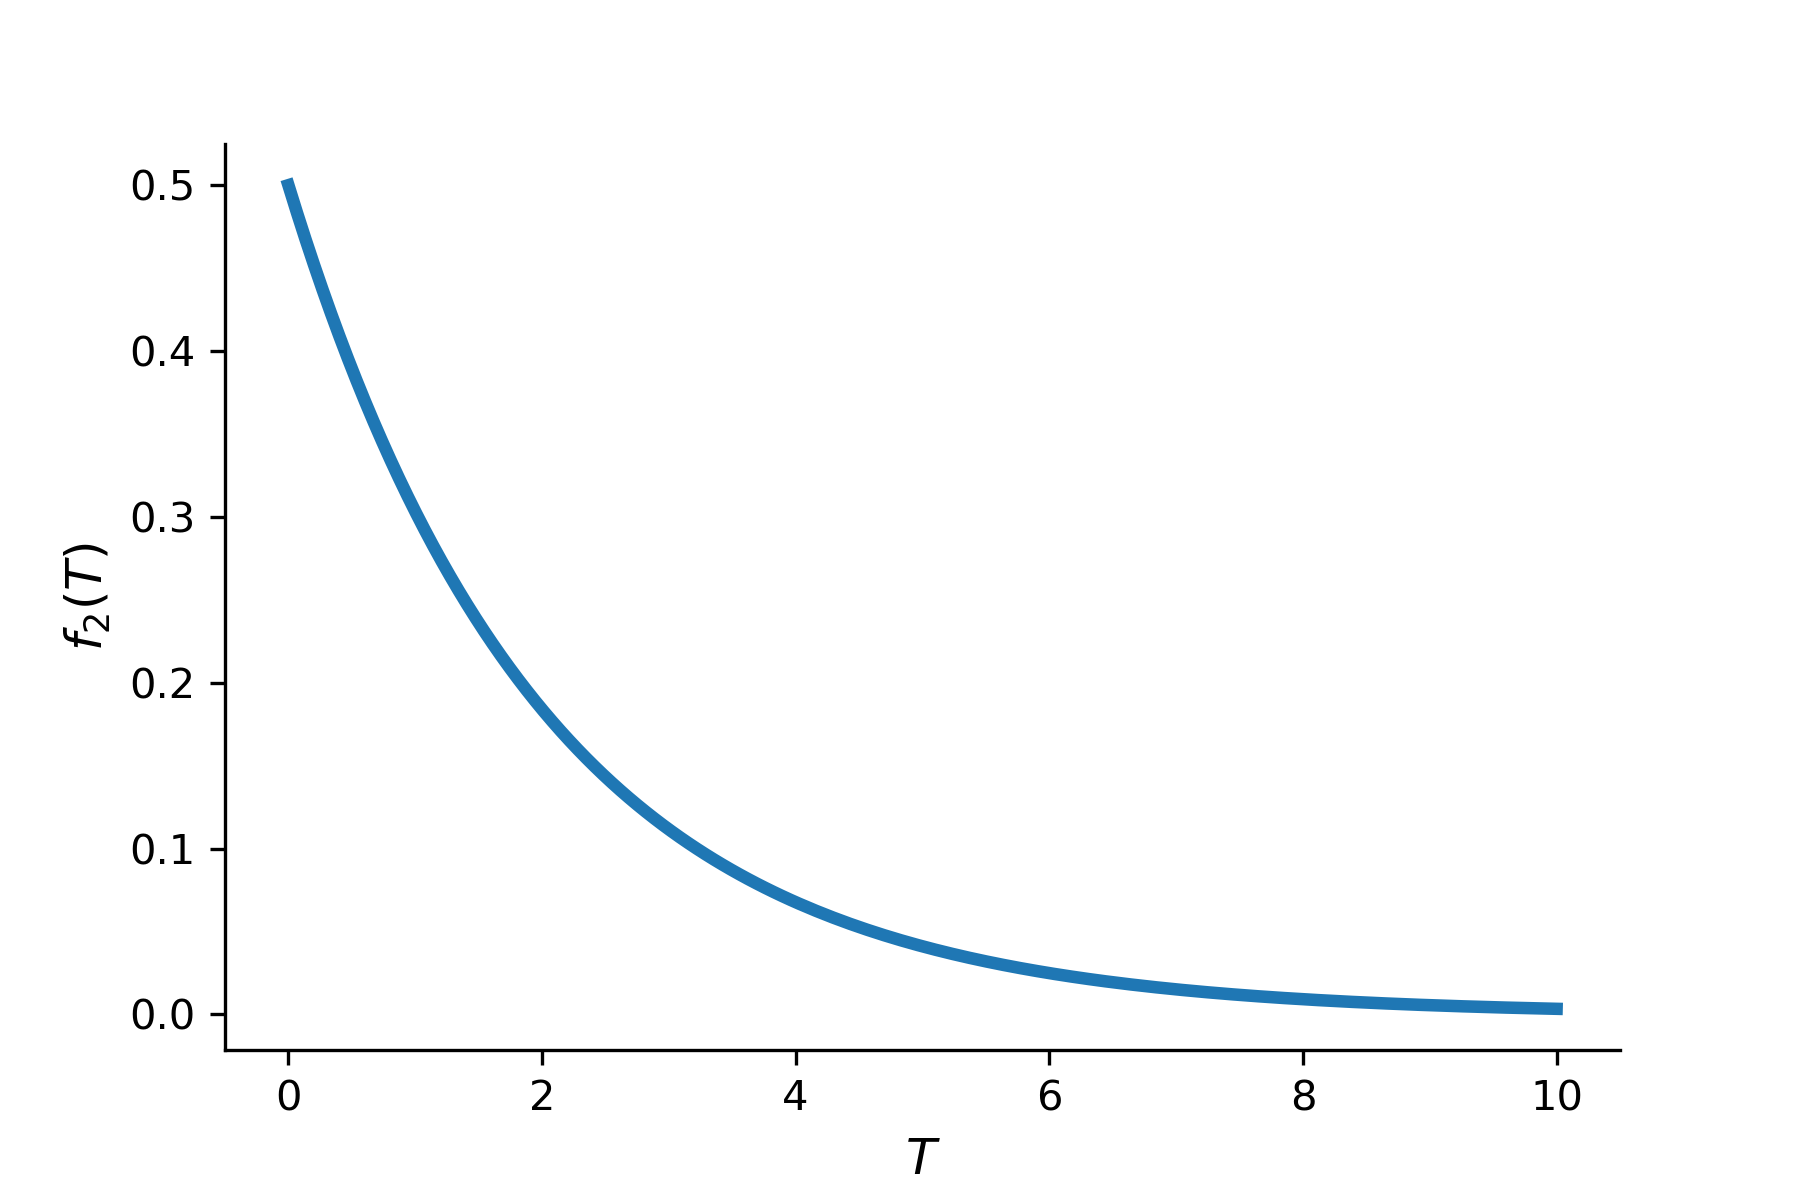
\includegraphics{material/chi-square-critical}}
\end{figure}
\end{frame}
%-------------------------------------------------------------------------------
%-------------------------------------------------------------------------------
\begin{frame}
\begin{figure}[htp]\centering
\caption{Density of $\chi^2(m - p)$}
\scalebox{0.75}{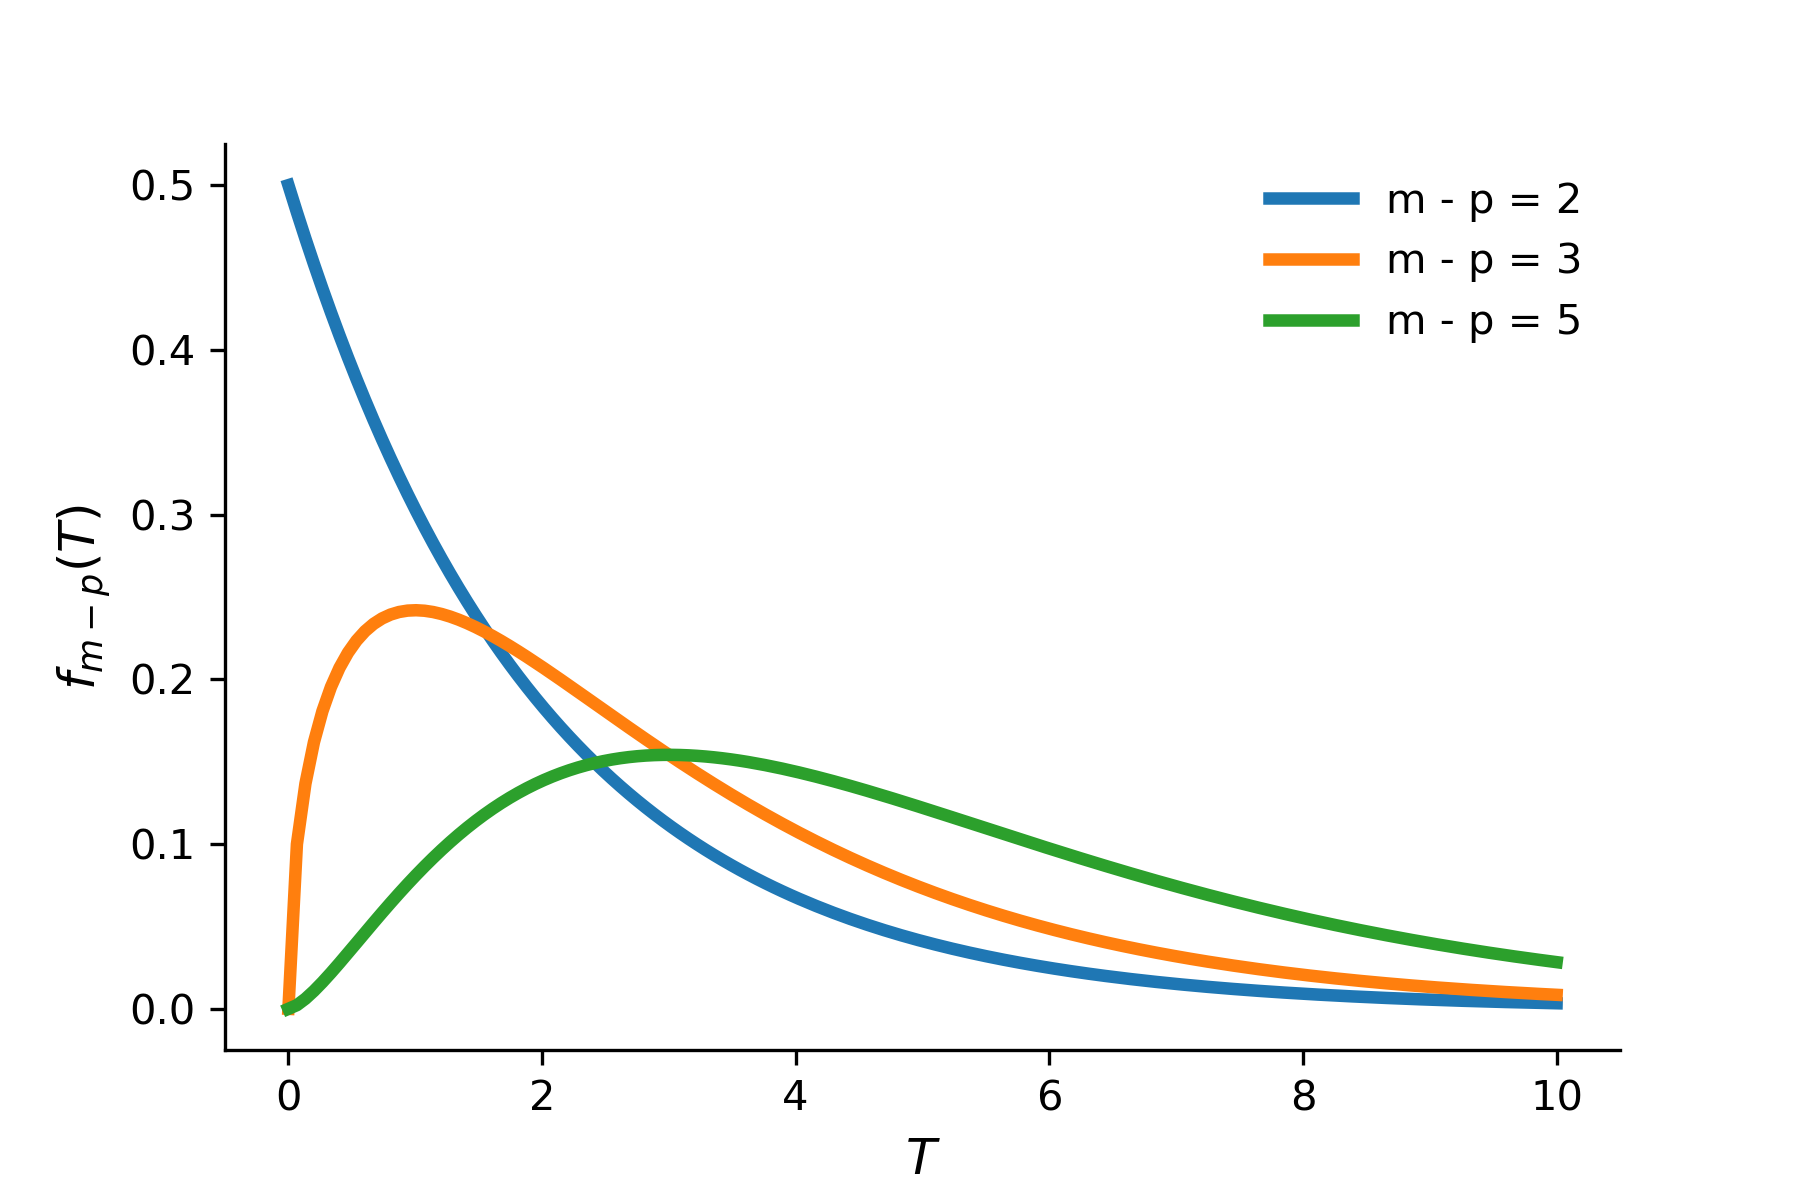
\includegraphics{material/chi-square-degrees}}
\end{figure}
\end{frame}
%-------------------------------------------------------------------------------
%-------------------------------------------------------------------------------
